\documentclass{article} % For LaTeX2e
\usepackage{nips14submit_e,times}
\usepackage{hyperref}
\usepackage{url}

% For figures
\usepackage{graphicx} % more modern
\usepackage{pstool}
\usepackage{caption}
\usepackage{subcaption}
\usepackage{lscape}
\usepackage{float}
%\usepackage{geometry}

% For citations
\usepackage{natbib}

% Nice colors
\usepackage{color,colortbl}

% Table related packages
\usepackage{multirow}
\usepackage{rotating}
% \newcommand\VRule[1][\arrayrulewidth]{\vrule width #1}

% Multiple columns
\usepackage{multicol}

% Enumerate items
\usepackage{enumitem}

% Math packages
\usepackage{amsmath,amsfonts,amssymb,amsthm,dsfont}
\usepackage{bm}
\usepackage{array,booktabs,xcolor}
\usepackage{color}

% Theorem environments
\newtheorem{theorem}{Theorem}
\newtheorem{definition}[theorem]{Definition}
\newtheorem{lemma}[theorem]{Lemma}
\newtheorem{proposition}[theorem]{Proposition}
\newtheorem{corollary}[theorem]{Corollary}

% Colors
\definecolor{LightGreen}{rgb}{0.87,0.90,0.82}
\definecolor{DarkGreen}{rgb}{0.60,0.73,0.35}
\renewcommand*\arraystretch{1.1}

% Proof sketch environment
\newenvironment{proofsketch}{\trivlist\item[]\emph{Proof Sketch}:}%
{\unskip\nobreak\hskip 1em plus 1fil\nobreak$\Box$
\parfillskip=0pt%
\endtrivlist}

\title{CS 267 Homework 1: Matrix Multiplication}

\author{
Karthik S. Narayan \\
Electrical Engineering and Computer Science\\
University of California, Berkeley\\
Berkeley, CA 94709 \\
\texttt{karthik.narayan@berkeley.edu} \\
\And
Charles A. Scudiere \\
Mechanical Engineering\\
University of California, Berkeley\\
Berkeley, CA 94709 \\
\texttt{cascudiere@berkeley.edu} \\
}

% The \author macro works with any number of authors. There are two commands
% used to separate the names and addresses of multiple authors: \And and \AND.
%
% Using \And between authors leaves it to \LaTeX{} to determine where to break
% the lines. Using \AND forces a linebreak at that point. So, if \LaTeX{}
% puts 3 of 4 authors names on the first line, and the last on the second
% line, try using \AND instead of \And before the third author name.

\newcommand{\fix}{\marginpar{FIX}}
\newcommand{\new}{\marginpar{NEW}}

\nipsfinalcopy % Uncomment for camera-ready version

\begin{document}

% Commonly used expressions
\newcommand{\dgemm}{\texttt{dgemm}}

% TODO commands
\newcommand\todo{\textcolor{red}{TODO}}
\newcommand\tocite{\textcolor{red}{CITE}}

\maketitle

\section{Optimizations Used and Attempted}
This section describes the approach we took in optimizing the \dgemm\; procedure,
which runs at an average $71\%$ of peak speed on an AMD MagnyCours under the
given test cases.
Concretely, we describe how we compute $C \leftarrow C + AB$. At a high level,
we (a) create auxiliary data structures that re-arrange and/or pad $A$, $B$,
and $C$, (b) employ blocking to multiply small blocks of $A$, $B$, and $C$,
where we (c) use SSE instructions with loop unrolling.

\subsection{Inner vs. Outer products}
\label{sec:ioproducts}
Originally, we coded up a standard ``inner-product-based'' matrix multiplication
algorithm. Unfortunately, we could not figure out a good way to perform
horizontal adds using SSE2, i.e. \texttt{\_mm\_hadd\_pd}. As such, we opted to go
for an ``outer-product-based'' method, noting that:
\begin{align}
  \label{eq:matmul}
  C = AB = \sum_{i}\sum_{j}A_i B^{(j)},
\end{align}
where $A_i$ denotes the $i$th row of $A$ and $B^{(j)}$ denotes the $j$th row of
$B$. In particular, the inner summand has the same size as $C$. To evaluate the
inner summand, we consider $4$ entries of $A_i$ and $4$ entries of $B^{(j)}$ at
a time, yielding a $4\times 4$ matrix that we can add to $C$. As an example,
iterating until $A_i$ and $B^{(j)}$ are covered yields a single summand
$A_i B^{(j)}$\footnote{This is just an example for clarity -- in reality, we do
  not do this, but rather iterate over blocks of A.}.

We load in the current values of the $4\times 4$ submatrix of $C$ that we
plan on updating; in particular, we use $8$ XMM registers for this.
In computing each $4\times 4$ contribution, we use $2$ XMM registers to store
the $4$ entries of $A_i$ exactly once. To easily broadcast $B^{(j)}$, we use
$4$ XMM registers for the $4$ entries of $B^{(j)}$, where each register contains
two of the same entry using the \texttt{\_mm\_load1\_pd} intrinsic. We compute
and add the associated multiplies to each of C's $8$ XMM registers. In total,
this procedure uses $8 + 4 + 2 = 14$ XMM registers, just under the total of $16$
provided with the AMD MagnyCours architecture.

To ensure that we work only with aligned SSE instructions and avoid fringe
cases, we pad $A$ and $C$ with zeros ahead of time; specifically, we pad
$A$ and $C$ with zeros so that the rows and columns are each multiples of $4$.
We do not pad $B$, since the \texttt{\_mm\_load1\_pd} intrinsic is unaligned.

\textbf{Testing Unrolling Sizes} In addition to working with $4\times 4$ matrices, we
experimented with $2\times 2$, $6\times 6$, and $8\times 8$ matrices.
Ultimately, $4\times 4$ worked the best, presumably because this uses just under
$16$ XMM registers.

\textbf{Testing AMD MagnyCours Pipelining} We also tried many possible
re-orderings of the various loads, adds, and multiplies involved in making the
$4\times 4$ updates. This made no measurable difference in runtimes, presumably
because the compiler automates this (we found out about this when spending time
in selecting compile flags).

\textbf{Testing Inner Product Methods} We originally implemented an
inner-product-based method, but were stuck on how to efficiently compute
reductions using SSE instructions (without SSE3). One major advantage of the
outer-product approach is that we do not have to resort to reduce operations.

\subsection{Memory Layout}
\label{sec:mem-layout}
One option in computing $C$ according to Equation~\eqref{eq:matmul} involves
(a) iterating over $i$, (b) iterating over $j$, and (c) in an inside loop,
computing $A_i B^{(j)}$. However, this does not take advantage of blocking
strategies. Instead, we make the $4\times 4$ updates as we iterate
over blocks of $A$ and rows of $B$ instead. We now describe how we lay out $A$,
$B$, and $C$, keeping this iteration strategy in mind. In general, all auxiliary
matrices are assigned on the stack, unless they are larger than
$1024 \times 1024$, in which case they are made on the heap.

Because we iterate over blocks of $A$, we store an
auxiliary matrix that stores entries of A columnwise block-by-block where each
block also has entries in column-major order. We make 16-byte-aligned memory
allocations on the stack, (a) to prepare for aligned SSE instructions and (b)
because matrix sizes tested are under 10 MB in size. We found that $68\times 68$
block sizes yielded good performance in practice. This procedure involves $4$
nested loops -- we tried all $24$ possible configurations and retained the best
ordering (see code for specifics).

Because we iterate over the rows of $B$, in processing
each block of $A$, we (a) copy the transpose of the block considered in $B$ into
an auxiliary matrix stored on the stack. Given $68\times 68$ blocks of $A$ and
$B$, we invoke the method described in Section~\ref{sec:ioproducts}.

We store $C$ in standard, column-major format. Recall that $A$, $B$, and $C$
are all padded to ensure that the side length is a multiple of $4$. In practice,
we could have also gone for a blocked implementation of $C$, but did not find
this necessary to get high performance (maybe blocking here would yield even
higher performance though).

\textbf{Testing Exhaustive Block Sizes.} We use one level
of blocking so as to improve the chances of matrix entries entering either the
L1 or the L2 cache. As we see later in this report, the lack of multiple layers
of blocking leads to decreased performance with increased matrix sizes, since
large matrices cannot fully fit into cached memory.

Instead of arbitrarily selecting a block size, we ran several experiments to determine the optimal block size. For each matrix size, we exhaustively tested all the block sizes with a multiple of $4$ up
to the matrix size. Rather than testing this via a \texttt{for}-loop over block sizes
directly within \texttt{benchmark.c}, we wrote a bash script which (1) replaced the
\texttt{\#define BLOCK\_SIZE} line with the appropriate block size. This was vital,
since directly coding this loop in C without generating the code would yield
substantially slower results (by 4\%); this is likely because in this latter case,
the block size would not be a compile-time constant. For robustness, we ran each
(block size, matrix size) tuple a total of four times to generate meaningful statistical data. In processing the output, we determined the best block size given the size of the matrix weighing in statistical averaging and assuming random "performance noise" to explain the variations in performance across each of the trail runs.

We present the results of these trials in Figures 1-5. Figures 1-4 summarize the
average performance for each individual array test size on Hopper, while Figure 5 summarizes
the performance using the selected block sizes chosen from the peak performance.

\clearpage
%\textwidth=8in
%\newgeometry{\textwidth=10cm,\textheight=10cm}
%\includepdf[pages={1,3,5}]{}
%\begin{center}
\begin{figure}
 %\centering
 \noindent
 \hspace*{-1.5in}
 \includegraphics[width=\paperwidth, page=1, trim={.25in 1.5in .25in 1.75in}]{"Block Size Performances".pdf} %\paperwidth \textwidth
 %\centering Figure 1 Performance vs. Average Block Size Graphs, Array sizes 31-191
 \caption{Performance vs. Average Block Size Graphs, Array sizes 31-191}
\end{figure}

\begin{figure}
 %\centering
 \noindent
 \hspace*{-1.5in}
 \includegraphics[width=\paperwidth, page=2, trim={.25in 1.5in .25in 1.75in}]{"Block Size Performances".pdf} %\paperwidth \textwidth
 %\centering Figure 2 Performance vs. Average Block Size Graphs, Array sizes 192-321
 \caption{Performance vs. Average Block Size Graphs, Array sizes 192-321}
\end{figure}

\begin{figure}
 %\centering
 \noindent
 \hspace*{-1.5in}
 \includegraphics[width=\paperwidth, page=3, trim={.25in 1.5in .25in 1.75in}]{"Block Size Performances".pdf} %\paperwidth \textwidth
 %\centering Figure 3 Performance vs. Average Block Size Graphs, Array sizes 417-767
 \caption{Performance vs. Average Block Size Graphs, Array sizes 417-767}
\end{figure}

\clearpage
One thing to notice about Figures 1-4 are the distinct dips in the performance at
certain block sizes. These dips seem to appear at consistently spaced intervals, for
all block sizes -- perhaps, this occurs due to cache misses (maybe the intervals
have to do with the AMD MagnyCours's cache line size?).

We can easily discern two trends from the figures. For block sizes of 97 and below,
increasing the block size greatly improves the performance until it asymptotes at
the array size. With increasing matrix sizes, another trend appears: we begin
to see inverted U patterns. For smaller block sizes, the required components likely
fit into the L1/L2 cache. Because we do not explore multiple levels of blocking, the
same components do not fully fit into the L1/L2 cache for larger matrix sizes, yielding
spillover into slow memory. This latter argument addresses why performance decreases
for larger matrices.

Analyzing the results in detail leads to determining the overall best block size
to choose. To determine the best sizes for a particular array size, the
statistical modes, averages, and individual test run performance were weighed.

Figures 1-4 show that, per matrix size, there is not a block size
that wins unequivocally -- rather, there is often a range of block sizes that typically
attains similar performance. Ultimately, we use the following ranges of block sizes:
for \texttt{lda}$\in [1, 32]$, we use a block size of $32$. For \texttt{lda}$\in [33, 97]$,
we use a block size of $52$. For \texttt{lda}$\in [98, 192]$, we use a block size of $68$.
For \texttt{lda}$\in [193, 639]$, we use a block size of $88$. For \texttt{lda}$\in [640, \infty]$,
we use a block size of $80$.

To ensure that \texttt{BLOCK\_SIZE} is still a compile-time constant, we employ
code generation; in particular, we define an auxiliary \texttt{square\_dgemm\_BLCK} that
has been defined in a pre-processor macro and contains most of the logic, assuming fixed block
size \texttt{BLCK}. The preprocessor macro allows us to then elegantly state the various
instances of the method (this simulates the concept of static-templating in C++).

A summary of the results with the selected block sizes are presented in Figure 5.
The performance for each of the optimized selected block sizes shown with three
distinct statistical analytics of the performance including the mean, median,
and mode of each test run at the selected optimal block size for each array size.

%\end{center}
%\restoregeometry

\begin{figure} % Note: figure is above the text.
 %\centering
 \noindent
 \hspace*{-1.5in}
 \includegraphics[width=\paperwidth, page=4, trim={.25in 7.75in .25in 1.75in}]{"Block Size Performances".pdf} %\paperwidth \textwidth
 %\centering Figure 4 Performance vs. Average Block Size Graphs, Array sizes 768-769
 \caption{Performance vs. Average Block Size Graphs, Array sizes 768-769}
\end{figure}

\clearpage
%\newgeometry{left=3cm,bottom=0.1cm}
%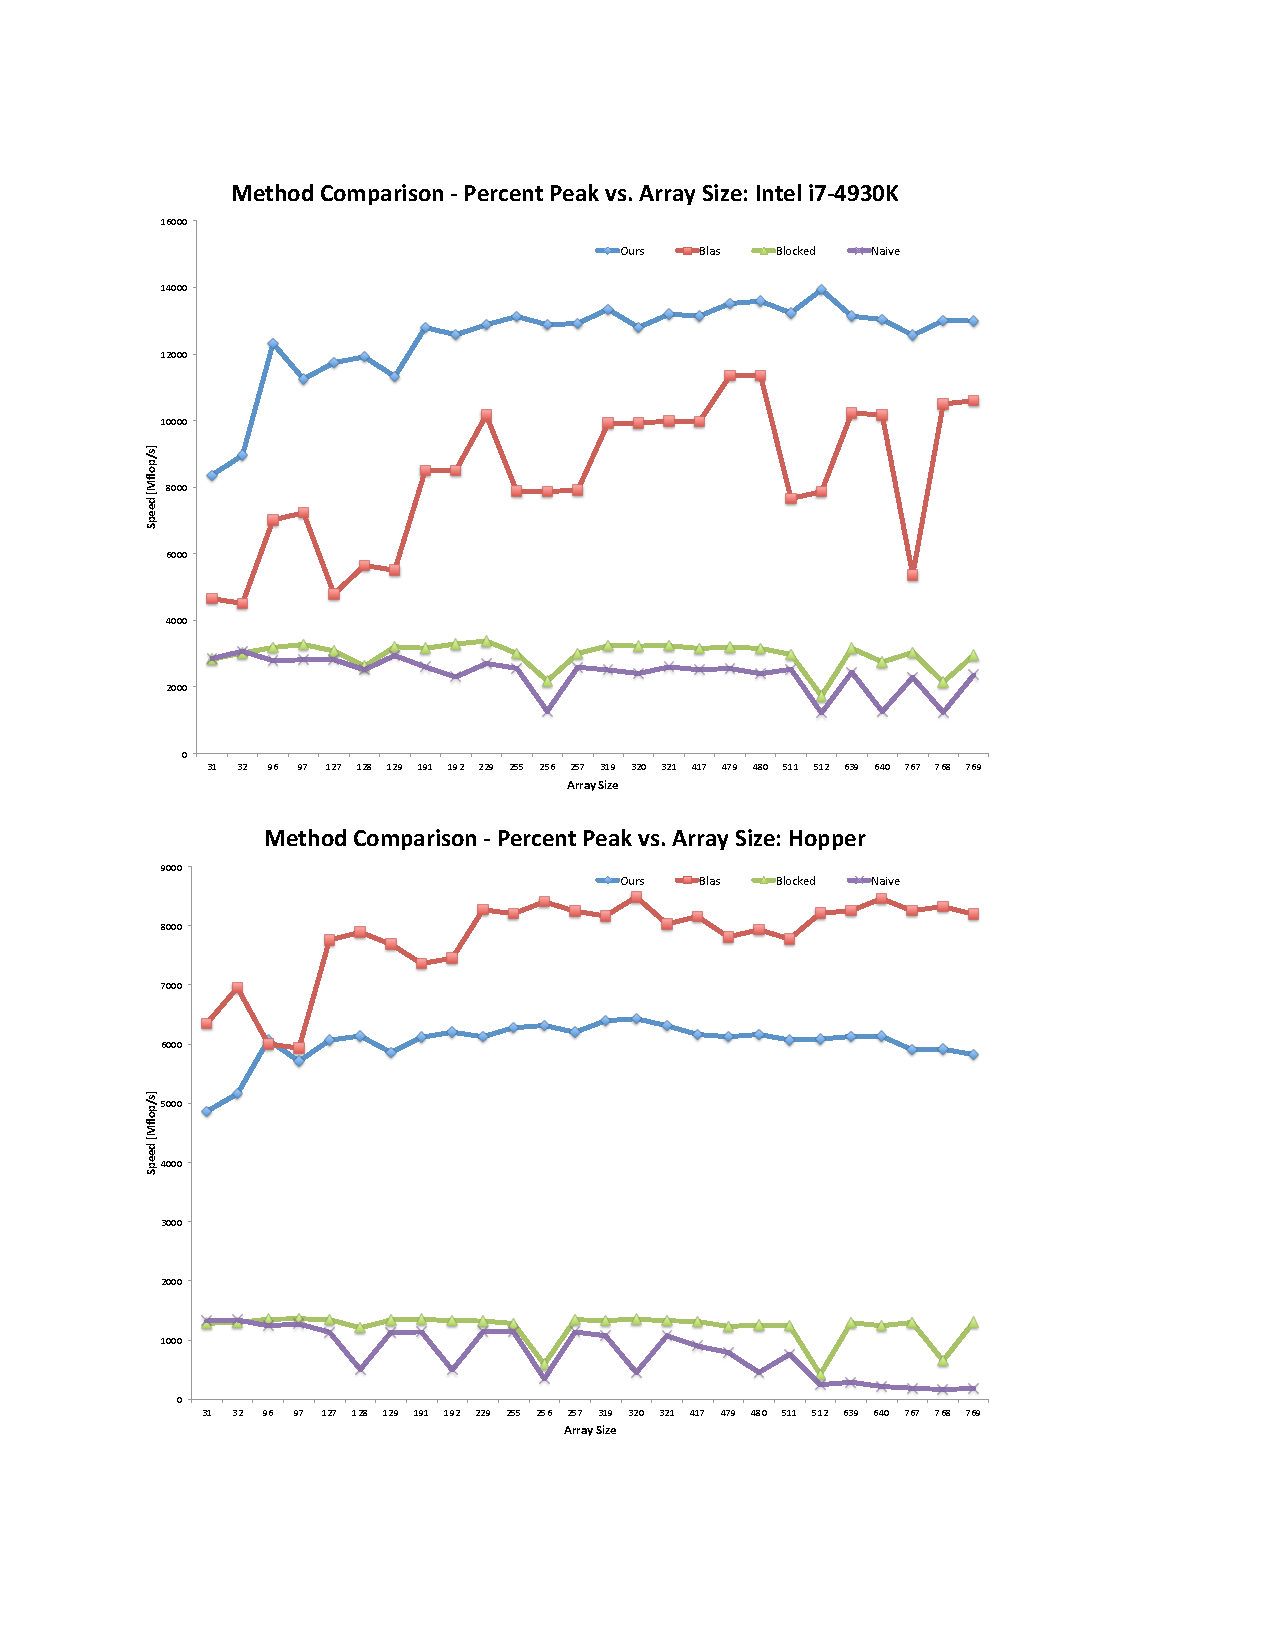
\includegraphics[scale=.5]{Method Comparison.pdf}
%\begin{landscape}
%\global\pdfpageattr\expandafter{\the\pdfpageattr/Rotate 90}
%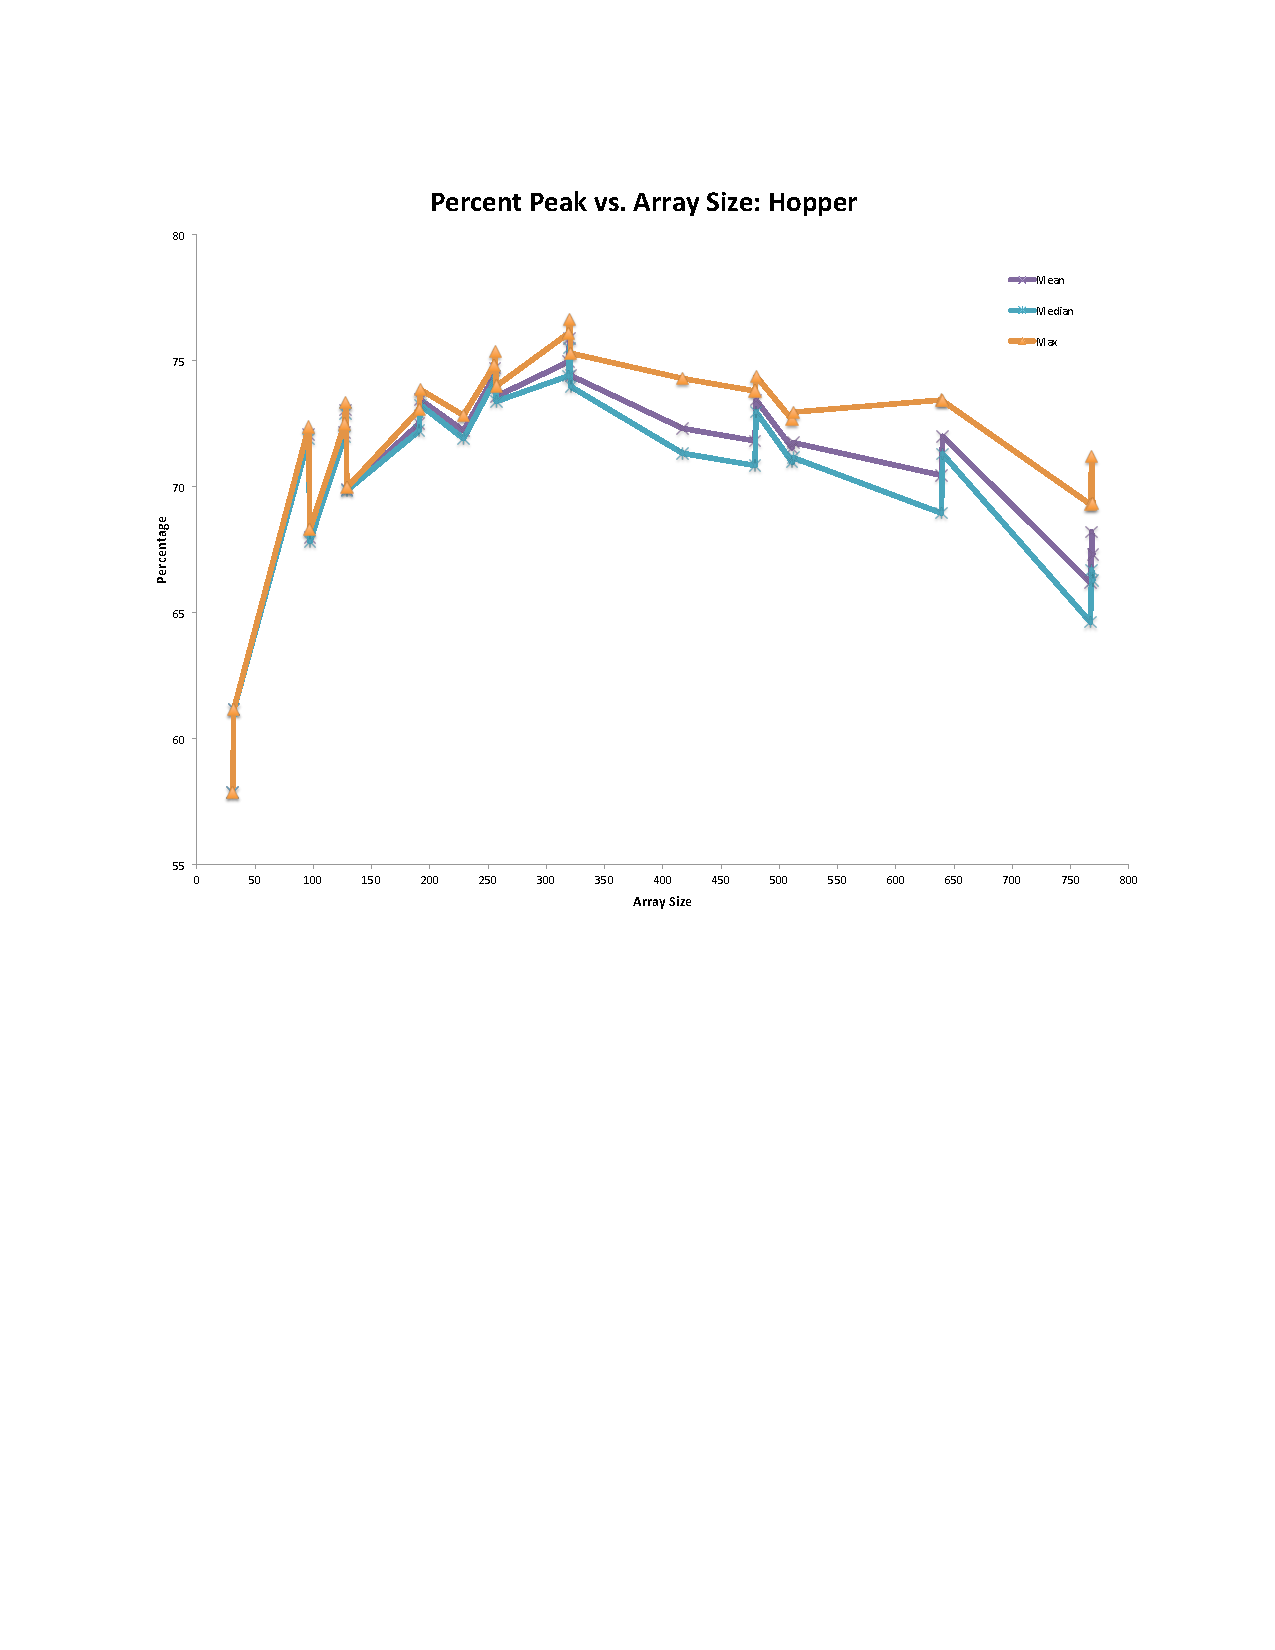
\includegraphics[scale=.5]{Selected Block Size Performance.pdf}
\begin{figure}
 %\centering
 \noindent
 \hspace*{-1.5in}
 \includegraphics[width=\paperwidth, page=1, trim={.25in 4.75in .25in 1.75in}]{"Selected Block Size Performance".pdf} %\paperwidth \textwidth
 %\centering Figure 6 Selected Block Performance, Array Size vs. Percentage
 \caption{Selected Block Performance, Array Size vs. Percentage}
\end{figure}
%\end{landscape}
% trim={<left> <lower> <right> <upper>}


\clearpage
\global\pdfpageattr\expandafter{\the\pdfpageattr/Rotate 0}

\subsection{Compile-Time-Known Block Sizes}
Due to fringes of matrices, there are regions in our code which prevent block
sizes from being known at compile time. To fix this, we auto-generated $8$
variants on the \texttt{do\_block} method, where each was a permutation on whether
each of $M$, $N$, or $K$ was known at compile time (if the variable is known, then
it would be set to the compile-time-constant block size). The goal here is that
if some subset of $M$, $N$, and $K$ are known at compile time, then the compiler
would be able to make further optimizations to the code (e.g., unforseen loop
unrolling). We then attempted to
select the appropriate method to run based on the information known.
Unfortunately, the if-statements required to select the appropriate method were
too slow for the benefits that this offered.

\subsection{Compiler Options}
We employ the following compiler options:
\begin{itemize}
  \item \texttt{-O2}: The supported options on hopper are \texttt{-O1}, \texttt{-O2},
    \texttt{-O3}, \texttt{-O4}, and \texttt{-Ofast}.
    We chose \texttt{-O2}, which was had a slightly better performance than \texttt{-Ofast}.
  \item \texttt{-march=native}: This option adds in further options that are
    specific to the native machine.
  \item \texttt{-funroll-loops}: This unrolls loops whose sizes are known at
    compile time.
  \item \texttt{-fsched-pressure}: This attempts to (1) eliminate execution
    stalls in the CPU pipeline when data is unavailable and (2) enables register
    pressure sensitive instruction scheduling before allocating registers.
    Ideally, this option minimizes register spillover.
  \item \texttt{-fsched-spec-load-dangerous}: To be honest, this flag sounded
    cool, so we decided to include it. It seemed to eke out a tenth of a percent
    performance, so why not include it. This allows for speculative motions of
    more load instructions.
\end{itemize}

We also experimented with \texttt{-funroll-all-loops} (slowed down performance in
comparison with \texttt{-funroll-loops}), \texttt{-ffast-math} (surprisingly
did not improve performance), \texttt{-fdata-sections} (slowed down performance),
and \texttt{-fbranch-target-load-optimize2} (made no difference).

We also experimented with \texttt{-fprofile-arcs}; after enabling this
flag and adding \texttt{-lgcov} to LDLIBS, we run our executable, which saves a
``.gcda'' file to disk. This file contains the various branch prediction
probabilities and other useful goodies, which we can then be used by future
executions of the code. Indeed, recompiling with the
\texttt{-fbranch-probabilities} flag, we unfortunately found that the resulting
code somehow ran slower (perhaps we didn't run something correctly).

\section{Testing on an Intel i7-4930K CPU}
We additionally tested our code on an Intel i7-4930K CPU to see how performance would
be impacted on an alternate machine build. Given that we heavily optimized our code and compile flags particularly
for the Hopper nodes, we had to make slight modifications to the makefile and the code; discussed
in Section~\ref{sec:mem-layout}, we allocate matrices smaller than $1024 \times 1024$
on the stack -- we had to decrease this size to $639\times 639$ to avoid stack overflows.
In order to run the provided BLAS benchmark, we had to link via \texttt{-lblas}. Other
than these two changes, we did not modify the code or other flags.

Shown in Figure 6 below, our code outperforms the native BLAS by a large factor.
In particular, the BLAS libraries were not installed from source, so there was no
opportunity for the compiler to specifically optimize the code to this machine.
However, our code was compiled on this machine, allowing the gcc compiler to specifically
optimize performance.

\clearpage
%\begin{landscape}
%\global\pdfpageattr\expandafter{\the\pdfpageattr/Rotate 90}
\begin{figure}  % Note: figure is above the text.
 %\centering
 \noindent
 \hspace*{-1.5in}
 \includegraphics[width=\paperwidth, page=1, trim={.25in 1.5in .25in 1.75in}]{"Method Comparison".pdf} %\paperwidth \textwidth
 %\centering Figure 5 Method Comparison, Array Size vs. Computation Speed
 \caption{Method Comparison, Percent Peak vs. Array Size}
\end{figure}
%\restoregeometry

%\end{landscape}

\small
\bibliographystyle{plain}
\bibliography{main}

\end{document}

